%%%%%%%%%%%%%%%%%%%%%%%%%%%%%%%%%%%%%%%%%%%%%%%%%%%%%%%%%%%%%%%%%%%%%%%%%%%%%%%%%%%%
%Do not alter this block of commands.  If you're proficient at LaTeX, you may include additional packages, create macros, etc. immediately below this block of commands, but make sure to NOT alter the header, margin, and comment settings here. 
\documentclass[12pt]{article}
 \usepackage[margin=1in]{geometry} 
\usepackage{amsmath,amsthm,amssymb,amsfonts, enumitem, fancyhdr, color, hyperref,comment, graphicx, environ,mathtools, bbm, tikz, setspace, cleveref,listings, dcolumn}
\usepackage{array, multirow, caption, booktabs}
\usepackage{lscape}
\usepackage{ mathrsfs }
\usetikzlibrary{matrix,positioning}
\tikzset{bullet/.style={circle,draw=black,inner sep=8pt}}
\DeclareMathOperator*{\argmax}{arg\,max}
\DeclareMathOperator*{\argmin}{arg\,min}
\DeclareMathOperator*{\Var}{\text{Var}}
\DeclareMathOperator*{\Cov}{\text{Cov}}

\DeclarePairedDelimiter\norm{\lVert}{\rVert}%
\newtheorem{theorem}{Theorem}
\newtheorem{lemma}[theorem]{Lemma}
\DeclareMathOperator{\eps}{\varepsilon}
\doublespacing
\DeclarePairedDelimiter\abs{\lvert}{\rvert}%
\pagestyle{fancy}
\setlength{\headheight}{65pt}
\newenvironment{problem}[2][Problem]{\begin{trivlist}
\item[\hskip \labelsep {\bfseries #1}\hskip \labelsep {\bfseries #2.}]}{\end{trivlist}}
\newenvironment{sol}
    {\emph{Solution:}
    }
    {
    \qed
    }


%%%%%%%%%%%%%%%%%%%%%%%%%%%%%%%%%%%%%%%%%%%%%%%%%%%%%%%%%%%%%%%%%%%%%%%%%%%%%%%%%


\usepackage{xcolor}
 
 


%%%%%%%%%%%%%%%%%%%%%%%%%%%%%%%%%%%%%%%%%%%%%

\rhead{Asha Bharadwaj, Caitlin Dutta, John Higgins, Alexis Smith\\Econ 899 \\ 28 November, 2022} 

%%%%%%%%%%%%%%%%%%%%%%%%%%%%%%%%%%%%%%%%%%%%


%%%%%%%%%%%%%%%%%%%%%%%%%%%%%%%%%%%%%%

\begin{document}
\begin{problem}{1}
\end{problem}
\begin{sol}
    We plot the error of the contraction mapping algorithm as well as the contraction method/Newton's method algorithm for 1985. They have a similar path until iteration 60 or so. Once the error drops below $\varepsilon = 1$, the error for Newton's method initially shoots up and then swiftly drops. Once it switches to Newton's method, the algorithm converges within a few iterations. Conversely, it takes the contraction mapping almost 80 additional iterations to converge from this point.
    \begin{center}
        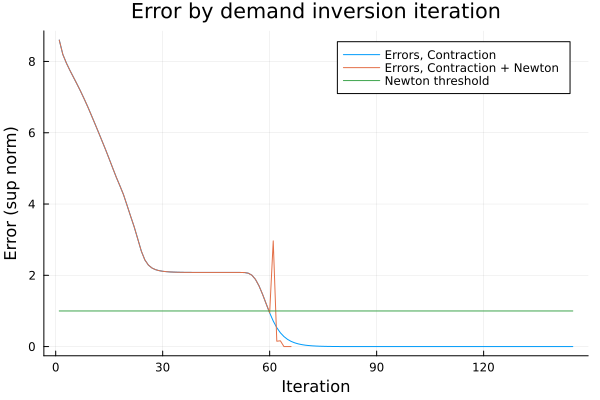
\includegraphics[scale=0.6]{error_plot.png}
    \end{center} 
\end{sol}
\begin{problem}{2}
\end{problem}
\begin{sol}
    We conduct a grid search for the optimal $\lambda_p \in [0,1]$ using the 2SLS weight matrix $W = (Z' Z)^{-1}$. We plot the objective function for each grid point below. The minimum objective function value of 234.7611 is attained at $\hat{\lambda}_p = 0.62$. 
    \begin{center}
        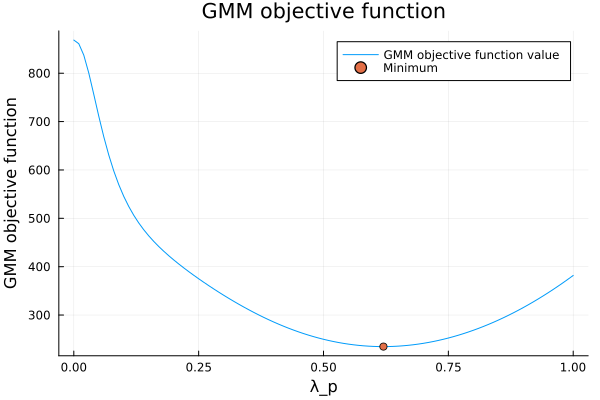
\includegraphics[scale=0.6]{gmmplot.png}
    \end{center}
\end{sol}
\begin{problem}{3}
\end{problem}
\begin{sol}
    Using $\hat{\lambda}_p = 0.62$, we construct the weight matrix $W = [(Z \xi)' ( Z \xi) ]^{-1}$, where $\xi = \rho(s, p \mid \hat{\lambda})$. We then use this to find the 2-step GMM estimator. We use LBFGS to minimize the GMM objective function and estimate that $\lambda_p = 0.5639$ with corresponding objective function value of 163.7396. We plot the new GMM objective function with the previous one below:
    \begin{center}
        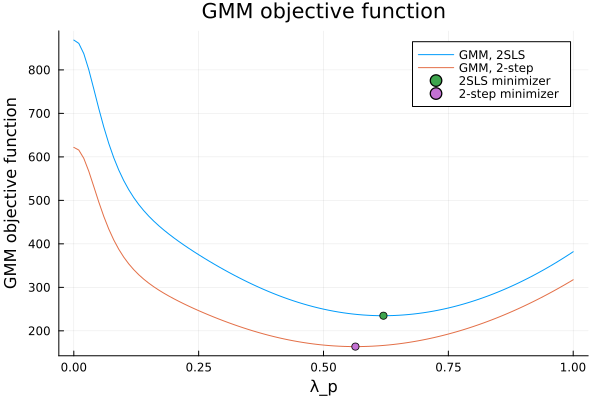
\includegraphics[scale=0.6]{gmm2step.png}
    \end{center}
\end{sol}
\end{document}